\documentclass[11pt]{article}
\usepackage[margin=1in]{geometry}
\usepackage{amsmath,amssymb}
\usepackage{graphicx}
\usepackage[colorlinks=true,linkcolor=blue,citecolor=blue,urlcolor=blue]{hyperref}


\title{Prefix-Path Bell Transport on IBM Quantum Hardware:\\
High-Resolution Replication, Comparative Geometry Dependence,\\
and Stress Tests of a Static--Dynamic Link\\
{\normalsize Version 2}}
\author{Lluis Eriksson\\ Independent Researcher\\ \texttt{lluiseriksson@gmail.com}}
\date{December 2025 (v1); July 2026 (v2)}

\begin{document}
\maketitle

\noindent\textbf{Editorial Status: Companion Note.}
This manuscript is a companion note in the coherence-maintenance program.
Role: experimental protocol note: controlled geometry, comparative rate
evidence, and stress tests of a static--dynamic link (RIP program context).
Program index: \url{https://ai.vixra.org/author/lluis_eriksson}

\begin{abstract}
This note reports a replicated, high-resolution Bell-transport experiment on
IBM Quantum superconducting hardware using a prefix-path protocol that
controls spatial heterogeneity across transport lengths. A single physical
qubit chain is fixed and increasing transport length $L$ is realized via
prefixes of that chain, so that $L$ changes depth while keeping qubits nested
rather than switching to different qubit subsets. We reconstruct the
Bell-state fidelity $F_{\Phi^+}(L)$ from Pauli correlators $E_{XX}, E_{YY},
E_{ZZ}$ and apply a minimal drift correction using interleaved full-$\Phi^+$
control blocks. Beyond a single-chain sweep, we perform a comparative
geometry test across three disjoint physical chains on the same backend: the
effective decay scale differs significantly across chains (with $>10\sigma$
separations under fit uncertainties), providing operational evidence that
the transport decay scale is geometry-dependent under fixed compilation
constraints. Motivated by the Rate Inheritance Principle (RIP) framing, we
also investigate whether a phase-sensitive static correlation metric measured
on idle chains can predict dynamical transport decay. A curated three-chain
set exhibits an ordering agreement between a static Ramsey-X nearest-neighbor
covariance metric and the transport decay scales $\mu$ measured on the same
chains; however, scale-up studies over $n=18$ randomly sampled chains and a
preregistered out-of-sample prediction test do not show statistically
significant monotone association under permutation testing. We interpret the
static--dynamic ordering agreement as conditional and geometry-specific,
while the geometry dependence of dynamical decay is robust. \emph{v2 adds:}
a fitting-choice caveat with a synthetically validated re-analysis pipeline
for future variant tables, a power bound showing the negative preregistered
test excludes a strong device-wide static--dynamic law (from published
quantities alone), an all-lengths rate proxy specification, small-sample and
estimator caveats, context references, and an offline re-analysis script
with documented schema for a future data revision.
\end{abstract}

\section{Scope and claim level}
This manuscript is an experimental companion note. Its primary contribution
is a reproducible protocol and dataset that isolates a dominant geometry
confound in short-depth transport experiments on superconducting QPUs.
We use the phrase \emph{operational rate inheritance} in a minimal
comparative sense: changing only the physical geometry (the qubit chain)
changes the effective decay scale extracted from an otherwise fixed protocol.
We also report phase-sensitive static measurements and stress tests of a
static--dynamic link motivated by the RIP program notes \cite{RIP0072,RIP0070}.
We do not claim a universal microscopic law relating a static correlation
envelope $f(\epsilon)$ to a Davies-rate envelope $\kappa(\epsilon)$ across
all regimes; the goal is operational: identify whether a practically
measurable static structure metric predicts dynamical transport decay
on-device. Geometry-dependent error heterogeneity and crosstalk on
superconducting devices are well documented
\cite{Sarovar2020,Tripathi2022}; the contribution here is a controlled
protocol that turns this into a quantitative comparative measurement under
fixed compilation constraints.

\section{Hardware, job metadata, and fixed physical geometry}
All experiments were executed on IBM Quantum \texttt{ibm\_fez} via IBM
Quantum Runtime (plan: open). The native entangling primitive exposed on the
relevant target subgraphs was \texttt{cz}. In the protocol description we use
logical gates such as CX and SWAP; these are compiled by Qiskit
\cite{Qiskit} to the backend basis under the fixed compilation constraints
described.

\paragraph{Single-chain high-resolution run (Figure~\ref{fig:hires}).}
Job ID: \texttt{d5aic8jht8fs73a5nrv0}. Shots per circuit: 2000. Repetitions
per $L$: $n_{\rm rep}=3$. Control mode: full-$\Phi^+$ drift blocks.

\paragraph{Comparative geometry run (Figure~\ref{fig:comparative}).}
Job ID: \texttt{d5aipuonsj9s73b7n65g}. Shots per circuit: 2000. Repetitions
per $L$: $n_{\rm rep}=3$. Three disjoint chains (length 8):
\begin{align*}
P_1 &= [130, 131, 138, 151, 152, 153, 154, 155],\\
P_2 &= [68, 69, 78, 89, 88, 87, 97, 107],\\
P_3 &= [0, 1, 2, 3, 4, 5, 6, 7].
\end{align*}

\paragraph{Curated static Ramsey-X scan (Figure~\ref{fig:stronglink}).}
Job ID: \texttt{d5ajj5rht8fs73a5p15g}. Shots per circuit: 2500. Idle times:
$T \in \{0, 2, 4, 6, 8\}\,\mu$s. (Same three chains as the comparative
transport run.)

\paragraph{Scale-up and stress tests (Figure~\ref{fig:scaleup} and
Table~\ref{tab:prereg}).}
Scale-up v2 job ID: \texttt{d5ak62jht8fs73a5pjbg} ($n=18$ random chains).
Edge-level static scan job ID: \texttt{d5ak8vbht8fs73a5pm5g} (per-edge
covariances). Preregistered screening job ID: \texttt{d5akfnrht8fs73a5psm0}
(select top/bottom groups by static metric). Preregistered dynamic test job
ID: \texttt{d5akj33ht8fs73a5pvt0} (out-of-sample prediction test on selected
chains).

\section{Protocol}
\subsection{Circuit family}
For each transport length $L$, we set $n = L+2$ and construct the following
circuit on $n$ qubits: prepare $\Phi^+$ on sites $(0,1)$ via H on qubit 0
followed by CX$(0,1)$; apply a SWAP chain transporting the second qubit from
site 1 to site $n{-}1$: SWAP$(1,2)\,$SWAP$(2,3)\cdots$SWAP$(n{-}2,n{-}1)$;
measure in Pauli bases $XX$, $YY$, $ZZ$ by applying standard basis-change
rotations on qubits 0 and $n{-}1$, followed by computational measurement on
those two qubits only. The prefix-path protocol fixes the physical mapping by
choosing a physical chain $P_{\rm phys}$ and using its prefix of length $n$
as the initial layout. Routing is disabled, and compilation uses optimization
level 0 to avoid structural rewriting.

\subsection{Fidelity estimator}
For each length $L$, we estimate correlators $E_{XX}, E_{YY}, E_{ZZ}$ from
parity outcomes and compute
\begin{equation}
F_{\Phi^+}(L) = \frac{1 + E_{XX}(L) - E_{YY}(L) + E_{ZZ}(L)}{4}.
\end{equation}

\subsection{Drift controls and correction}
To reduce slow drift, we interleave full-$\Phi^+$ control blocks at $L=0$
(three Pauli bases) and use a minimal control-referenced correction:
\[
F_{\rm corr} = F_{\rm raw} - \bigl( F_{\rm ctrl,near} - \bar F_{\rm ctrl} \bigr).
\]
This corrects coarse drift at the level of the control schedule; it is not
intended as a full time-series model. \emph{(Added in v2)} $F_{\rm corr}$ is
an affine-corrected estimator and is not constrained to $[0,1]$; no clipping
is applied, so that averages remain unbiased.

\subsection{Uncertainty reporting}
For each $L$, we run $n_{\rm rep}=3$ repetitions and report the mean and
standard error of the mean (SEM) across repetitions. \emph{(Added in v2)}
With $n_{\rm rep}=3$ the SEM itself carries large relative uncertainty
(2 degrees of freedom); confidence intervals built from these SEMs should
use Student-$t$ factors, and the fit-based uncertainties quoted below
inherit this caveat. The scale-up analyses instead use multinomial
bootstrapping of shot outcomes, which does not suffer from this
small-$n_{\rm rep}$ issue.

\section{Results I: single-chain high-resolution sweep}
Figure~\ref{fig:hires} shows the replicated single-chain sweep (prefix-path)
with error bars. A descriptive fit of the form $F(L) = A e^{-\mu L} + B$ can
be used as a compact summary; fitted parameters are model-dependent and
should be treated as descriptive rather than as direct observables.

\begin{figure}[t]
\centering
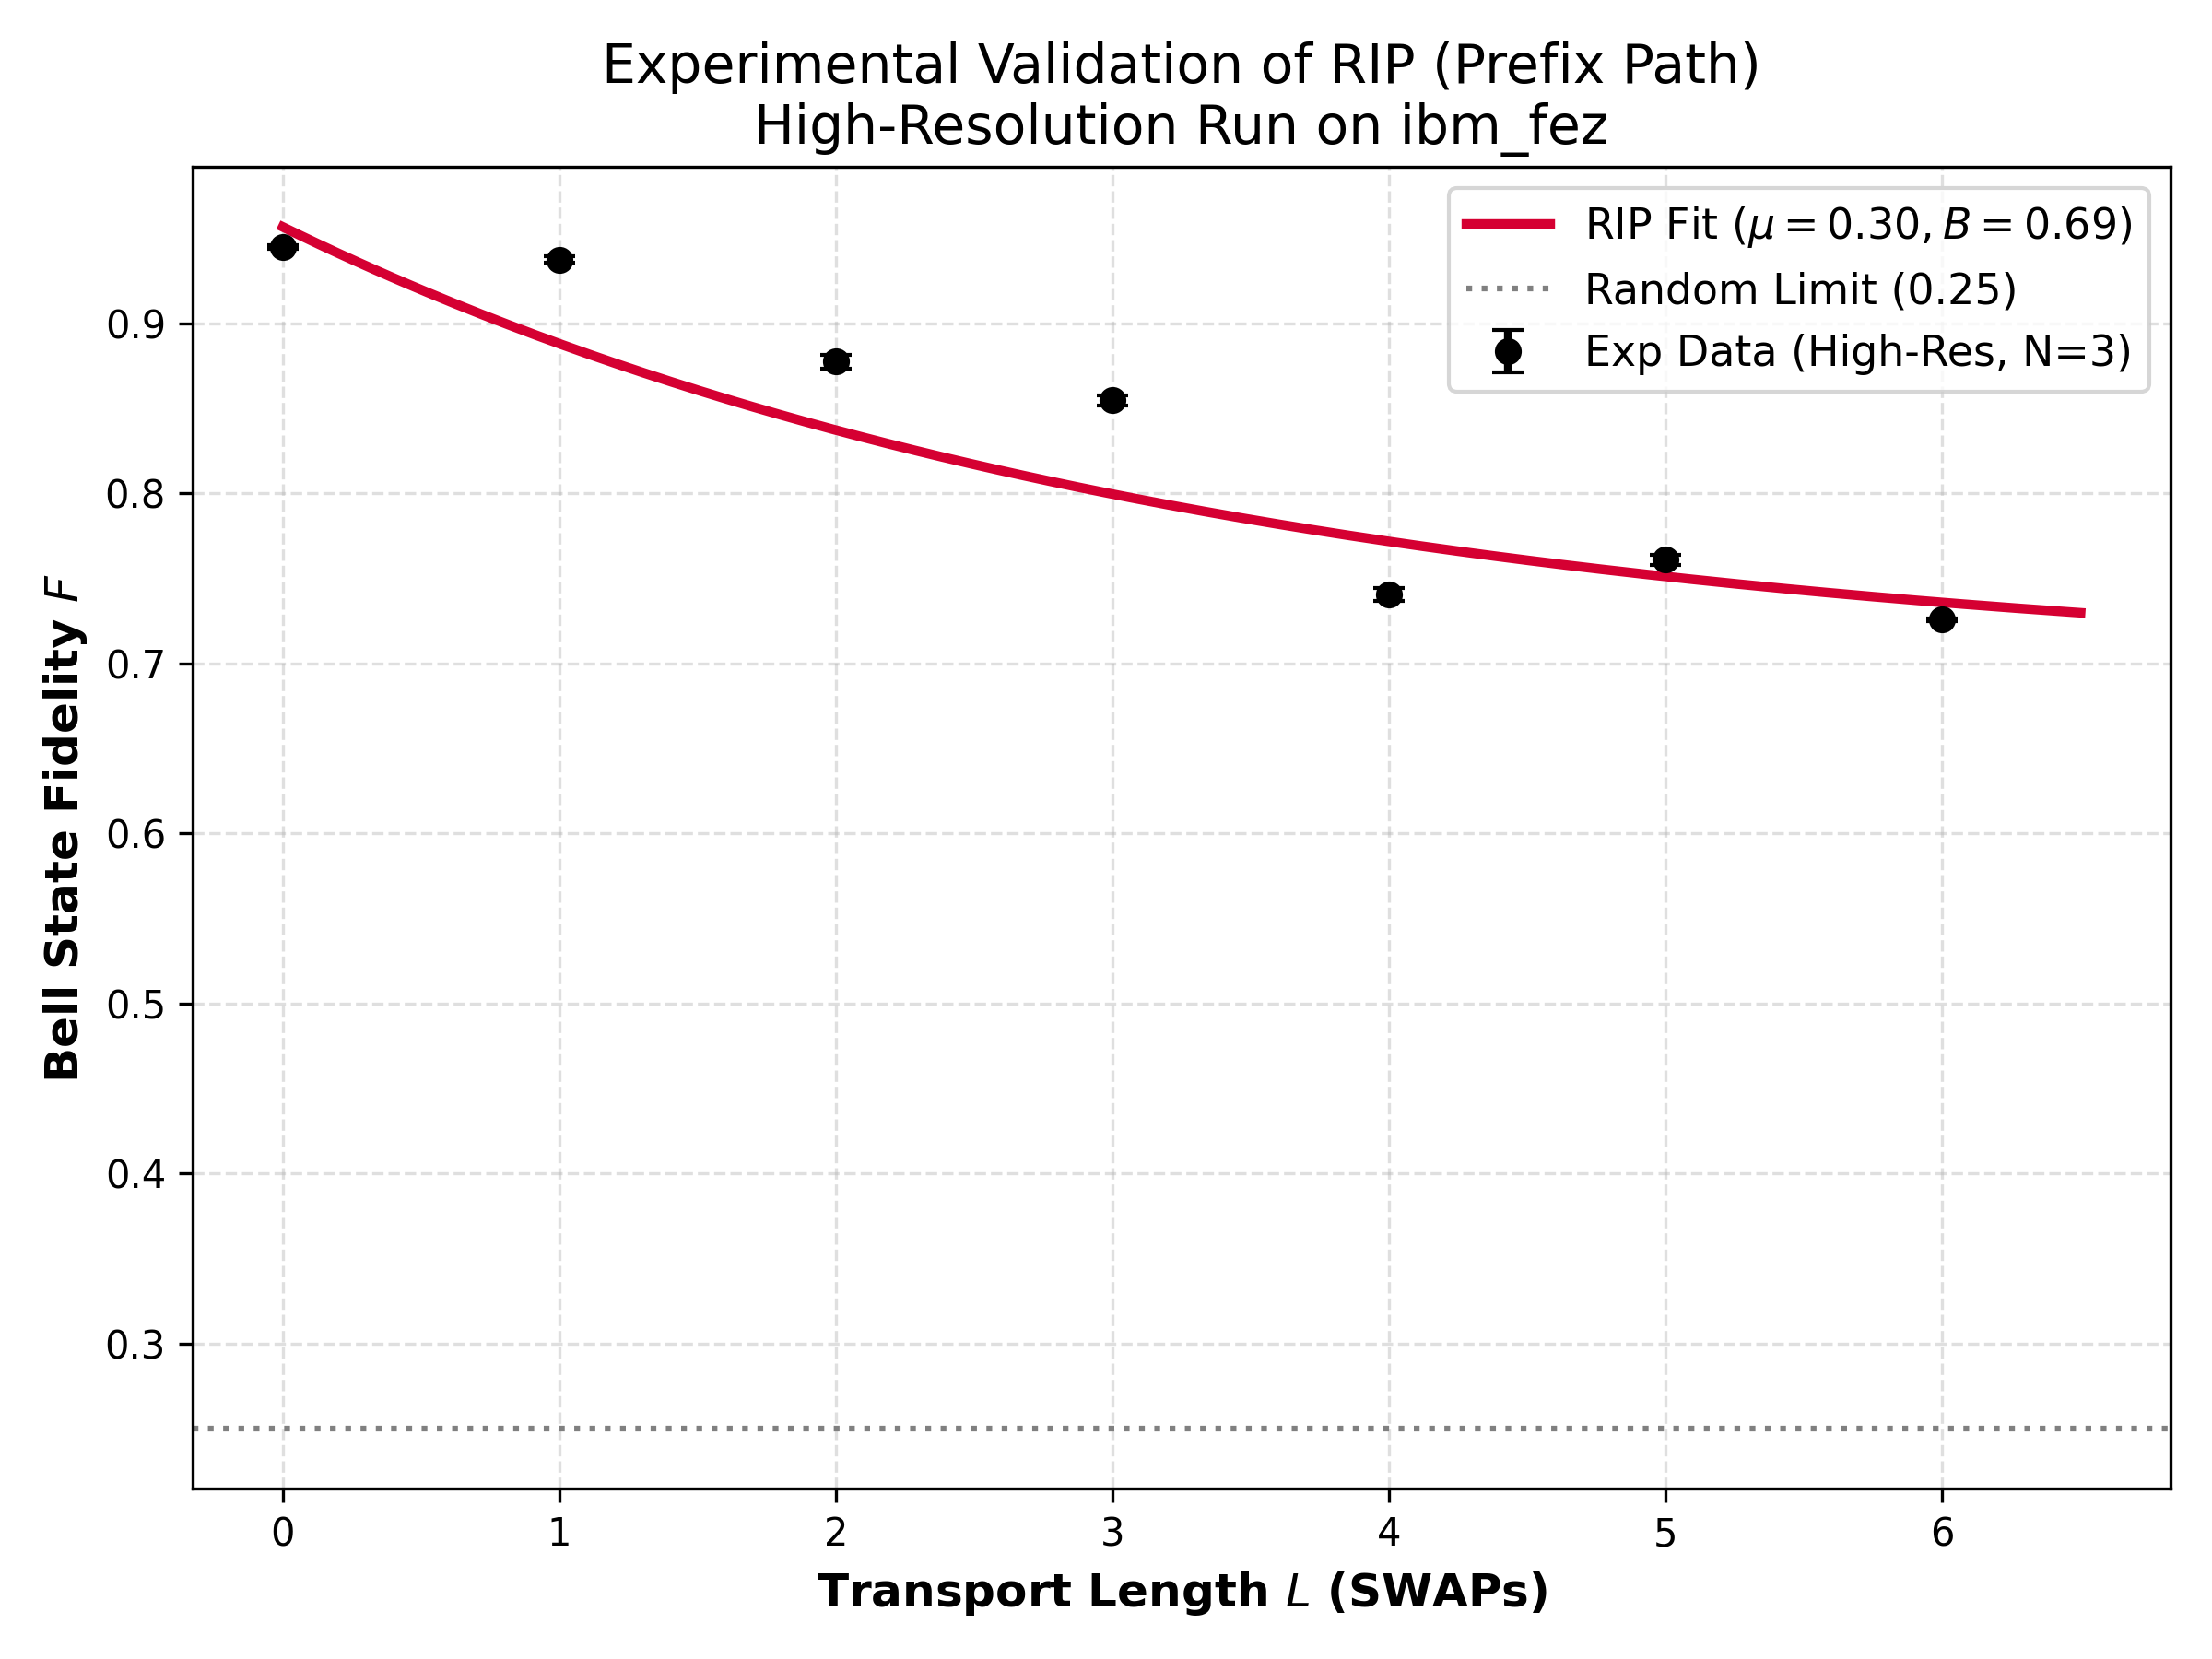
\includegraphics[width=0.8\textwidth]{rip_final_defense.png}
\caption{High-resolution prefix-path Bell transport on \texttt{ibm\_fez}
(single-chain run).}
\label{fig:hires}
\end{figure}

\section{Results II: comparative geometry test (operational rate inheritance)}
To test whether the effective decay scale depends on physical geometry rather
than being a universal constant of the protocol, we repeated the sweep on
three disjoint physical chains under identical compilation constraints.

\subsection{Fit protocol for the comparative test}
For the comparative test we summarize each chain by an effective decay scale
$\mu$ using
\begin{equation}
F(L) = B_{\rm fix} + (F_0 - B_{\rm fix})\, e^{-\mu L}.
\label{eq:fit}
\end{equation}
Here $B_{\rm fix}$ is defined operationally for each chain as the empirical
mean of the two largest-$L$ fidelity points available on that chain; we then
fit $(F_0, \mu)$ by weighted nonlinear least squares (weights
$1/\sigma_{\rm SEM}(L)^2$). This stabilizes inference when the asymptote is
not identifiable in the sampled $L$ range.

\subsection{Observed geometry dependence}
The extracted decay scales (baseline variant, as in v1) are
\[
\mu_1 = 0.2224 \pm 0.0182,\qquad
\mu_2 = 0.5398 \pm 0.0186,\qquad
\mu_3 = 0.3014 \pm 0.0068.
\]
Key separations:
\[
\mu_2 - \mu_1 = 0.3174 \pm 0.0261,\qquad
\mu_2 - \mu_3 = 0.2384 \pm 0.0198,
\]
corresponding to $>10\sigma$ differences under the reported uncertainties.
The quoted $\pm$ are fit standard errors from the weighted nonlinear
least-squares procedure; they do not include systematic/model uncertainty.
Because the three chains are disjoint, the corresponding datasets are
approximately independent at the hardware level.

\subsection{Fitting-choice caveat (added in v2)}
$B_{\rm fix}$ (asymptote from the two largest-$L$ points) is a modeling
choice that can bias the absolute $\mu$ when the asymptote is not reached in
the sampled range. Synthetic-data validation of the re-analysis pipeline
shipped with this note (\texttt{verification/0105/reanalyze\_0105.py},
\texttt{--demo} mode; Section~\ref{sec:repro}) confirms both effects: on
synthetic chains with known ground truth, the v1 $B_{\rm fix}$ variant
overestimates $\mu$ by $\sim 25\%$, while the \emph{ordering} of
well-separated decay scales is preserved across the v1 choice, a free-$B$
three-parameter fit, and $B_{\rm fix}=1/4$ (the depolarizing floor), with
$\ge 7\sigma$ minimal separation. For the on-device dataset the
corresponding variant table requires the archived per-$L$ fidelities and is
deferred to a data revision. The headline geometry claim of this note
therefore rests on the v1 fit uncertainties quoted above, read as
\emph{ordering and separation} rather than absolute $\mu$ values, with the
explicit caveat that quoted errors exclude model-choice systematics.

\begin{figure}[t]
\centering
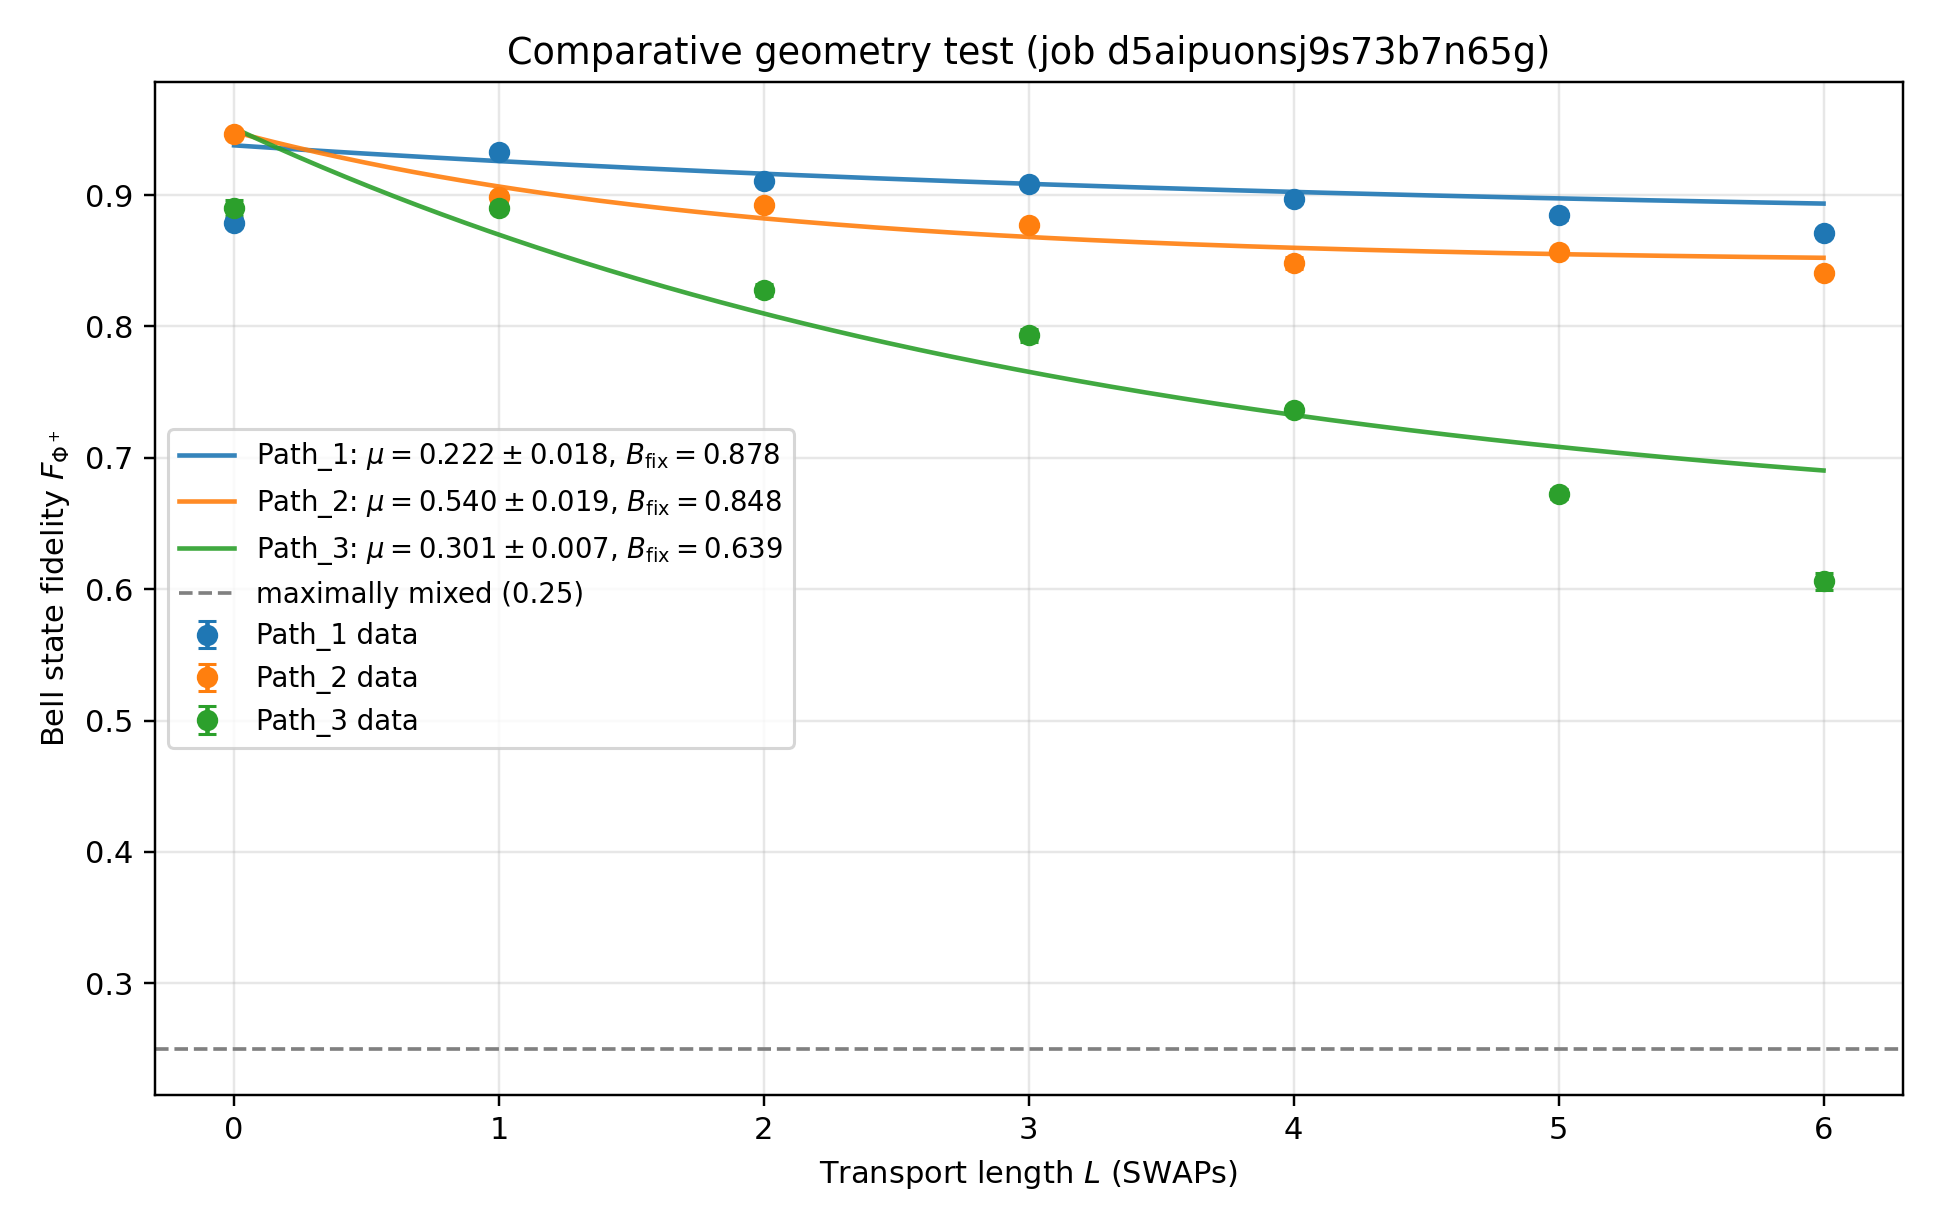
\includegraphics[width=0.8\textwidth]{rip_comparative_plot_v3_fixB.png}
\caption{Comparative geometry test on \texttt{ibm\_fez}. Error bars are SEM
over $n_{\rm rep}=3$ repetitions per $L$. Curves show the weighted fit
Eq.~\eqref{eq:fit} with the v1 baseline $B_{\rm fix}$.}
\label{fig:comparative}
\end{figure}

\section{Calibration snapshot and descriptive static-to-dynamic check}
We queried a backend-reported calibration snapshot for the three chains
(timestamp: 2025-12-31 11:29 UTC). Reported values are simple averages over
qubits ($T_1$, readout error) and over adjacent edges (mean two-qubit gate
error) along each chain.

\begin{table}[h]
\centering
\caption{Backend-reported calibration snapshot for the three disjoint chains.}
\begin{tabular}{ccccc}
\hline
Path & $\mu$ & $T_1$ ($\mu$s) & Avg 2Q err. & Readout err. \\
\hline
1 & $0.2224 \pm 0.0182$ & 133.5 & 0.0026 & 0.0181 \\
2 & $0.5398 \pm 0.0186$ & 116.0 & 0.0029 & 0.0177 \\
3 & $0.3014 \pm 0.0068$ & 182.2 & 0.0078 & 0.0158 \\
\hline
\end{tabular}
\end{table}

The calibration snapshot does not uniquely determine $\mu$; this is expected,
since $\mu$ is a protocol-level effective parameter aggregating multiple
error sources. As an auxiliary descriptive check, Figure~\ref{fig:lambda}
plots drift-corrected fidelities against the composite proxy
$\Lambda_{2Q}(L) = N_{2Q}(L)\, \epsilon_{2Q}$, where $N_{2Q}(L)$ is the
observed two-qubit gate count per transpiled circuit and $\epsilon_{2Q}$ the
mean reported two-qubit gate error along the chain.

\begin{figure}[t]
\centering
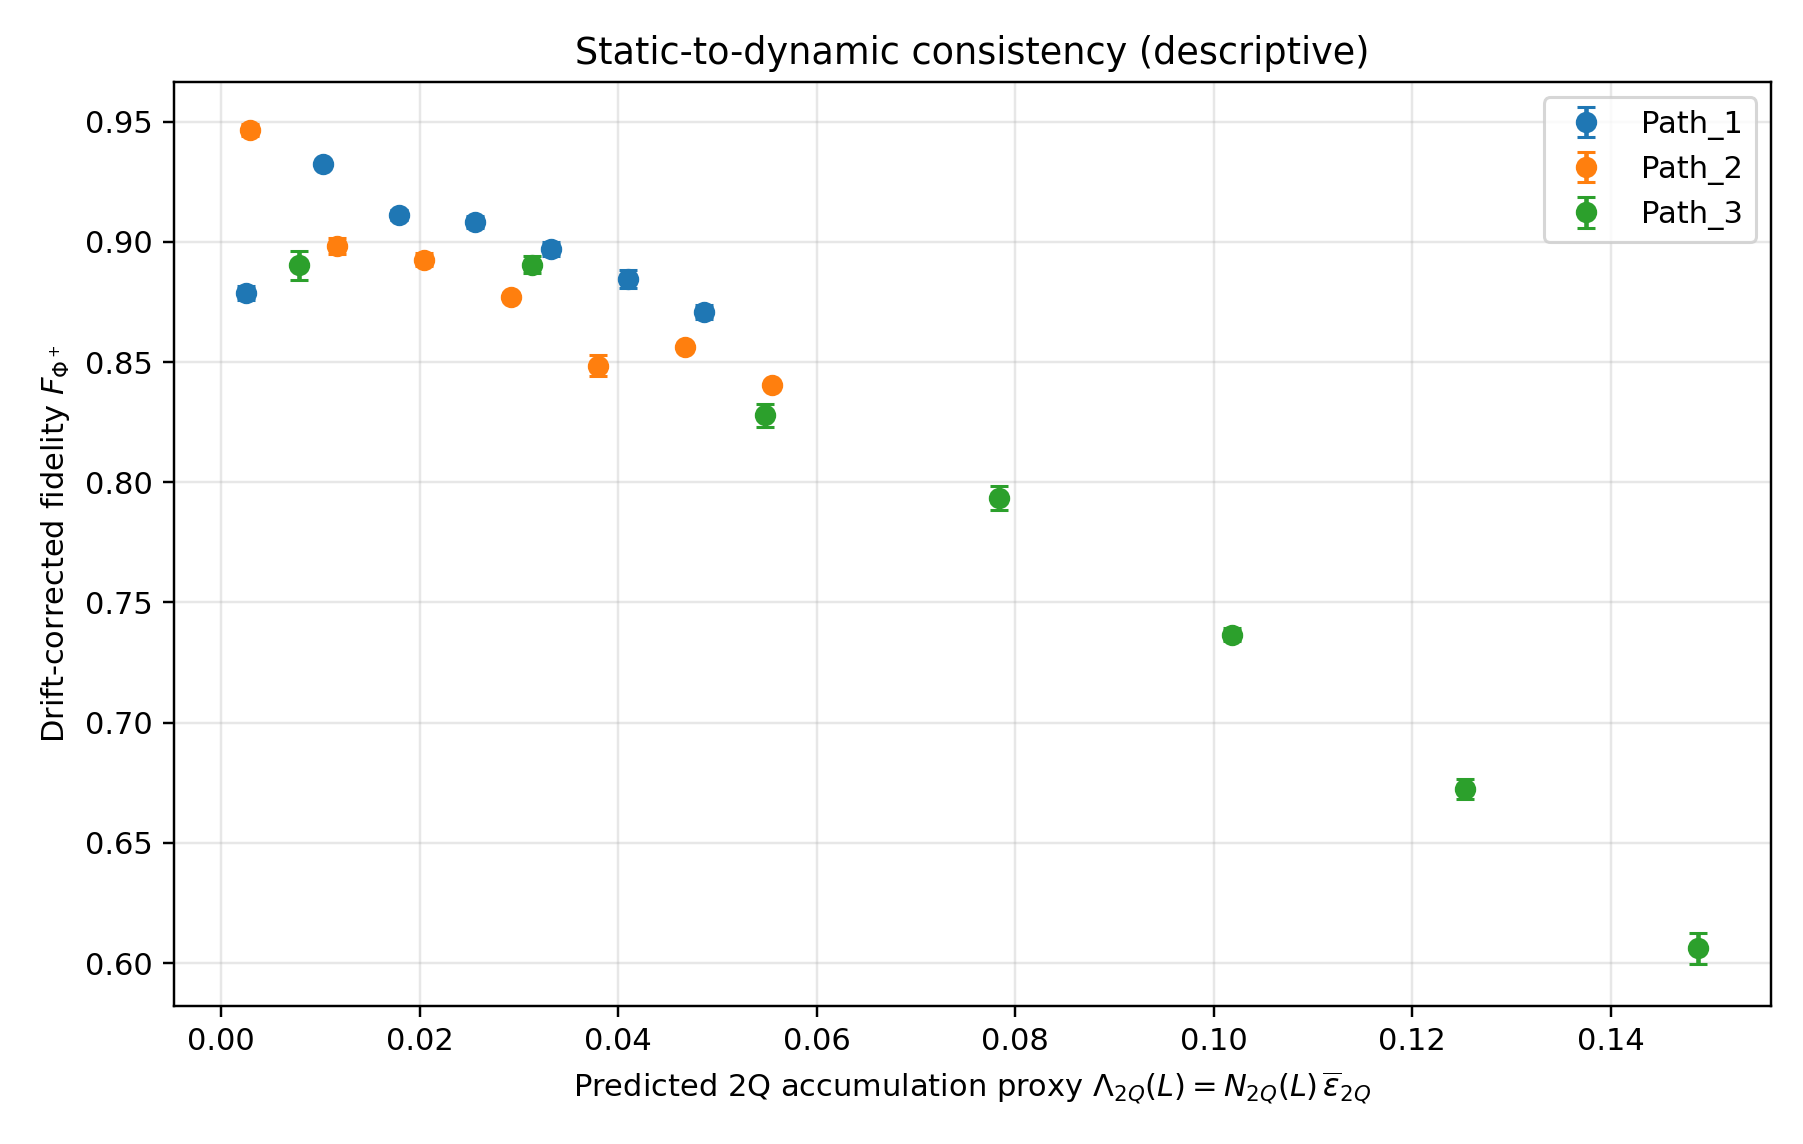
\includegraphics[width=0.7\textwidth]{fig3_lambda2q_0105.png}
\caption{Descriptive static-to-dynamic consistency check: drift-corrected
mean fidelity vs $\Lambda_{2Q}(L)$. A consistency check, not a universal
predictive model.}
\label{fig:lambda}
\end{figure}

\section{Static measurements and a candidate static--dynamic ordering link}
\subsection{Motivation (RIP bridge)}
In the RIP framing \cite{RIP0072}, a central hinge is whether a practically
measurable static structure observable can predict a dynamical decay penalty
extracted from an active protocol. Prior notes emphasize that inheritance is
conditional and can fail in specific regimes \cite{RIP0070}. Here we test an
operational version on-device using a phase-sensitive static probe
(Ramsey-X).

\subsection{Curated three-chain static--dynamic ordering agreement}
On each 8-qubit chain we prepare $\lvert + \rangle^{\otimes 8}$, idle for a
duration $T$, and measure in the $X$ basis. From the resulting bitstring
distribution we compute nearest-neighbor covariances
$C^{(X)}_{i,i+1}(T) = \langle X_i X_{i+1}\rangle_T - \langle X_i\rangle_T
\langle X_{i+1}\rangle_T$, aggregated as
$S_{\rm stat}(T) = \frac{1}{7}\sum_{i=0}^{6} \lvert C^{(X)}_{i,i+1}(T)\rvert$,
and use the SPAM-corrected scalar
$S_{\rm stat,corr} = \overline{S_{\rm stat}(T \ge 2\,\mu{\rm s})} -
S_{\rm stat}(0)$. Figure~\ref{fig:stronglink} plots $\mu$ against
$S_{\rm stat,corr}$ for the curated three-chain set; the ordering agrees
(Path1 $<$ Path3 $<$ Path2 in both).

\begin{figure}[t]
\centering
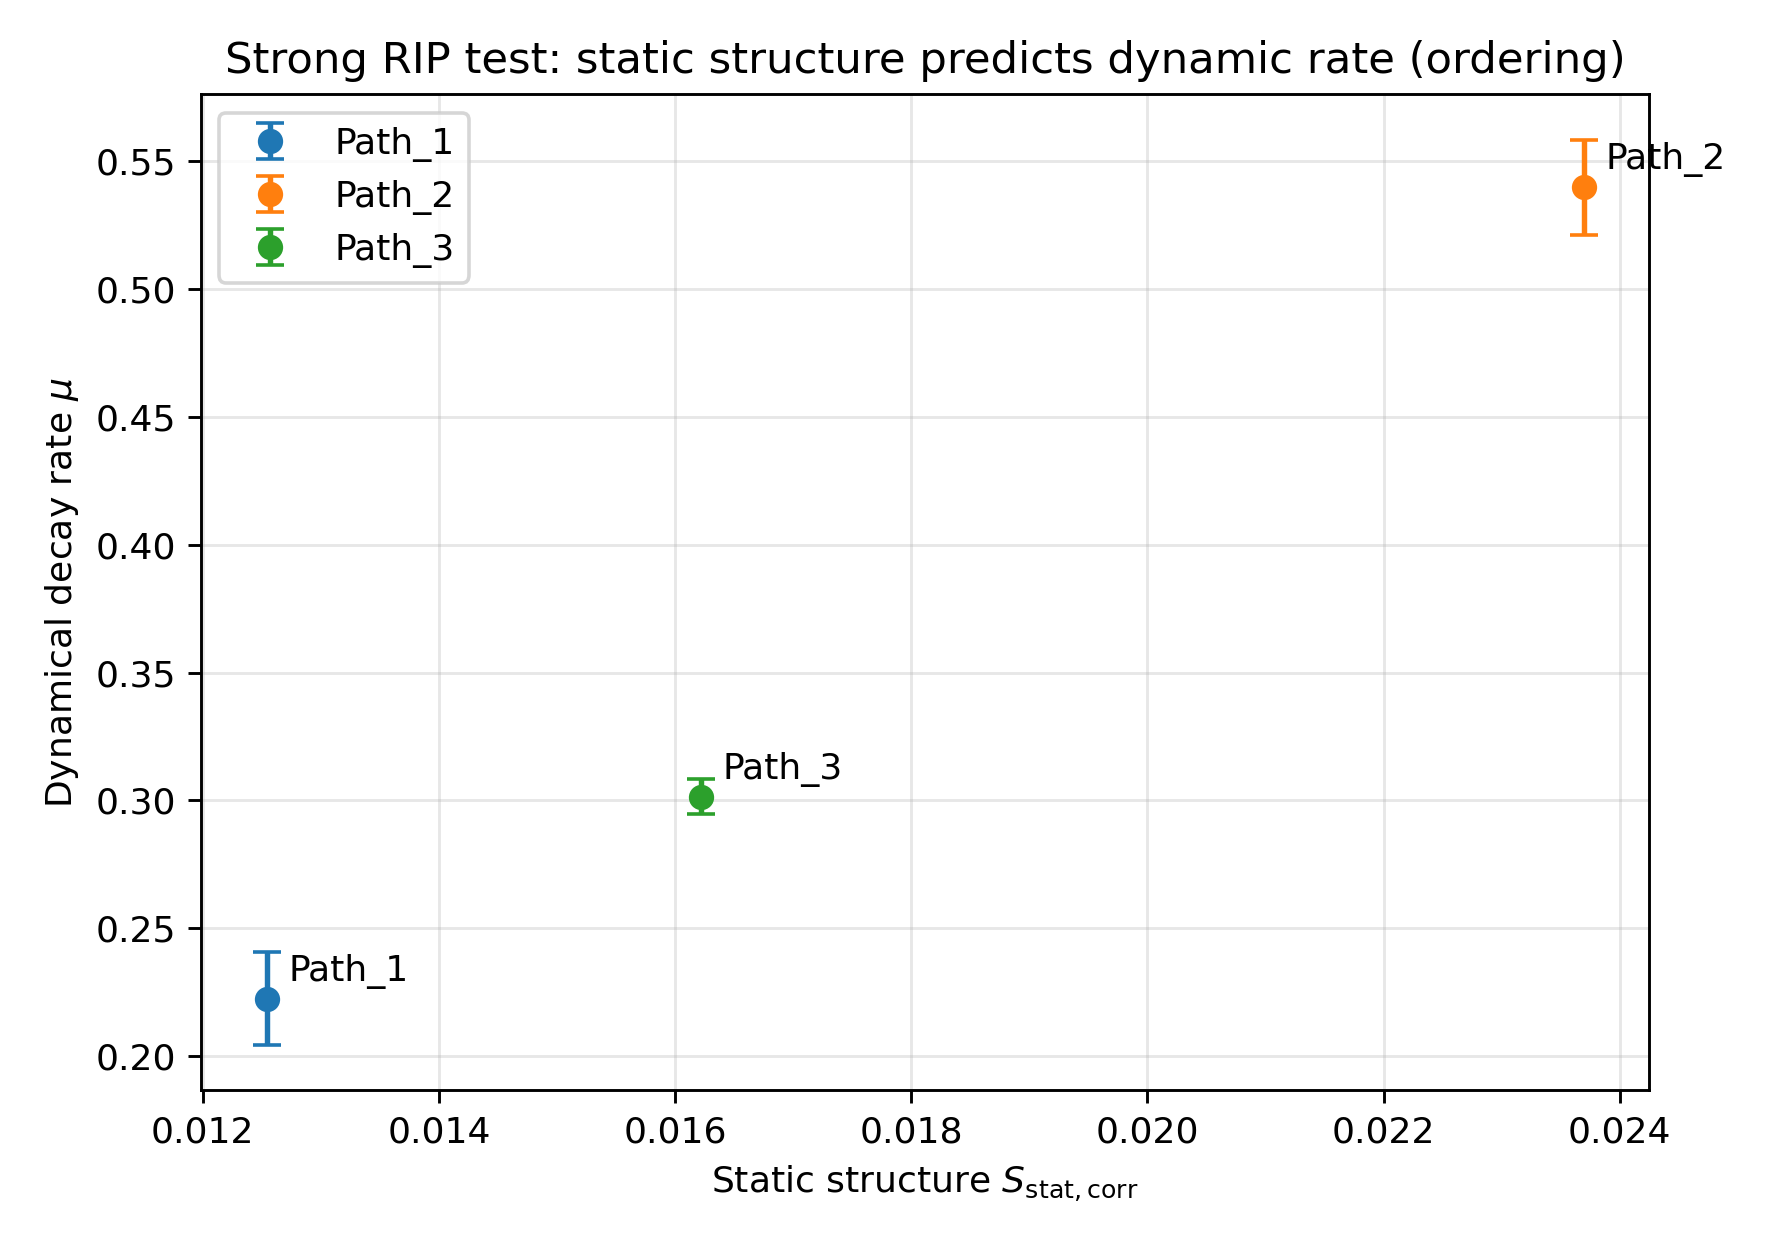
\includegraphics[width=0.7\textwidth]{rip_strong_link.png}
\caption{Curated three-chain ordering: $S_{\rm stat,corr}$ vs $\mu$.}
\label{fig:stronglink}
\end{figure}

\begin{table}[h]
\centering
\caption{Curated three-chain summary on \texttt{ibm\_fez}.}
\begin{tabular}{ccc}
\hline
Path & $S_{\rm stat,corr}$ & $\mu$ \\
\hline
1 & 0.012543 & $0.222437 \pm 0.018202$ \\
3 & 0.016221 & $0.301424 \pm 0.006824$ \\
2 & 0.023694 & $0.539802 \pm 0.018637$ \\
\hline
\end{tabular}
\end{table}

\subsection{Scale-up stress tests and preregistered prediction test (negative)}
\label{sec:negative}
To evaluate whether the static metric predicts dynamical decay more broadly,
we performed stress tests on randomly sampled chains and a preregistered
out-of-sample prediction test.

\paragraph{Dynamic rate proxies.} To avoid sensitivity to long-length
saturation, v1 defined the short-length proxy
\begin{equation}
\mu_{04} := \frac{1}{4} \ln\!\left( \frac{1 - F_{\Phi^+}(4)}{1 - F_{\Phi^+}(0)} \right).
\end{equation}
\emph{(Added in v2)} Since $L \in \{0,2,4,6\}$ was measured, an
all-lengths proxy $\mu_{\rm all}$ -- the slope of a least-squares fit of
$\ln(1 - F)$ over all four lengths -- is specified in the re-analysis script
as a cross-check on the two-point choice; its evaluation on the archived
per-$L$ fidelities is deferred to a data revision.

\paragraph{Scale-up v2 ($n=18$ random chains).} A Spearman rank test with a
permutation $p$-value yields no statistically significant association (job
\texttt{d5ak62jht8fs73a5pjbg}): $\rho \approx 0.23$, two-sided permutation
$p \approx 0.35$ (Figure~\ref{fig:scaleup}).

\paragraph{Edge-restricted static metric (negative).} Restricting the static
metric to the SWAP edges used at $L=4$ does not improve association (job
\texttt{d5ak8vbht8fs73a5pm5g}): $\rho \approx 0.18$, $p \approx 0.46$.

\paragraph{Preregistered out-of-sample prediction test (negative).} Using a
static screening run on $n=30$ random chains, we selected $k=5$ chains with
the smallest and largest values of the simplified metric
$S_{\rm stat}(6\,\mu{\rm s}) - S_{\rm stat}(0)$ (screening job
\texttt{d5akfnrht8fs73a5psm0}), then measured $\mu_{04}$ on these 10 chains
with $n_{\rm rep}=3$ (dynamic job \texttt{d5akj33ht8fs73a5pvt0}). The
preregistered statistic $\Delta := \overline{\mu_{04}}\,|_{\rm HIGH} -
\overline{\mu_{04}}\,|_{\rm LOW}$ was observed to be $\Delta \approx -0.0014$
with permutation $p_{\rm 1\text{-}sided} \approx 0.50$ (two-sided $p = 1.0$).

\paragraph{Power of the negative test (added in v2).} A negative result is
informative only relative to the effects it could have detected. For the
preregistered design ($k=5$ per group, one-sided $\alpha=0.05$, power
$0.80$) the minimum detectable effect is
\[
\Delta_{\rm MDE} = (z_{0.95} + z_{0.80})\, \sigma_{\rm chain}\sqrt{2/k}
\approx 1.57\, \sigma_{\rm chain},
\]
where $\sigma_{\rm chain}$ is the between-chain dispersion of $\mu_{04}$
(numerical evaluation deferred to the data revision). A bound follows from
published quantities alone: for an effect of the size suggested by the
curated three-chain set (spread $\approx 0.3$ in $\mu$) to have escaped
detection, one would need $\sigma_{\rm chain} \gtrsim 0.19$ -- roughly
$60\%$ of the mean $\overline{\mu_{04}} \approx 0.33$, implausibly large
for chains on a single backend. The design was therefore adequately powered
against a \emph{strong} device-wide static--dynamic law; the null result
rules that out, while remaining compatible with a weak or
mechanism-specific association below $\Delta_{\rm MDE}$.

\begin{figure}[t]
\centering
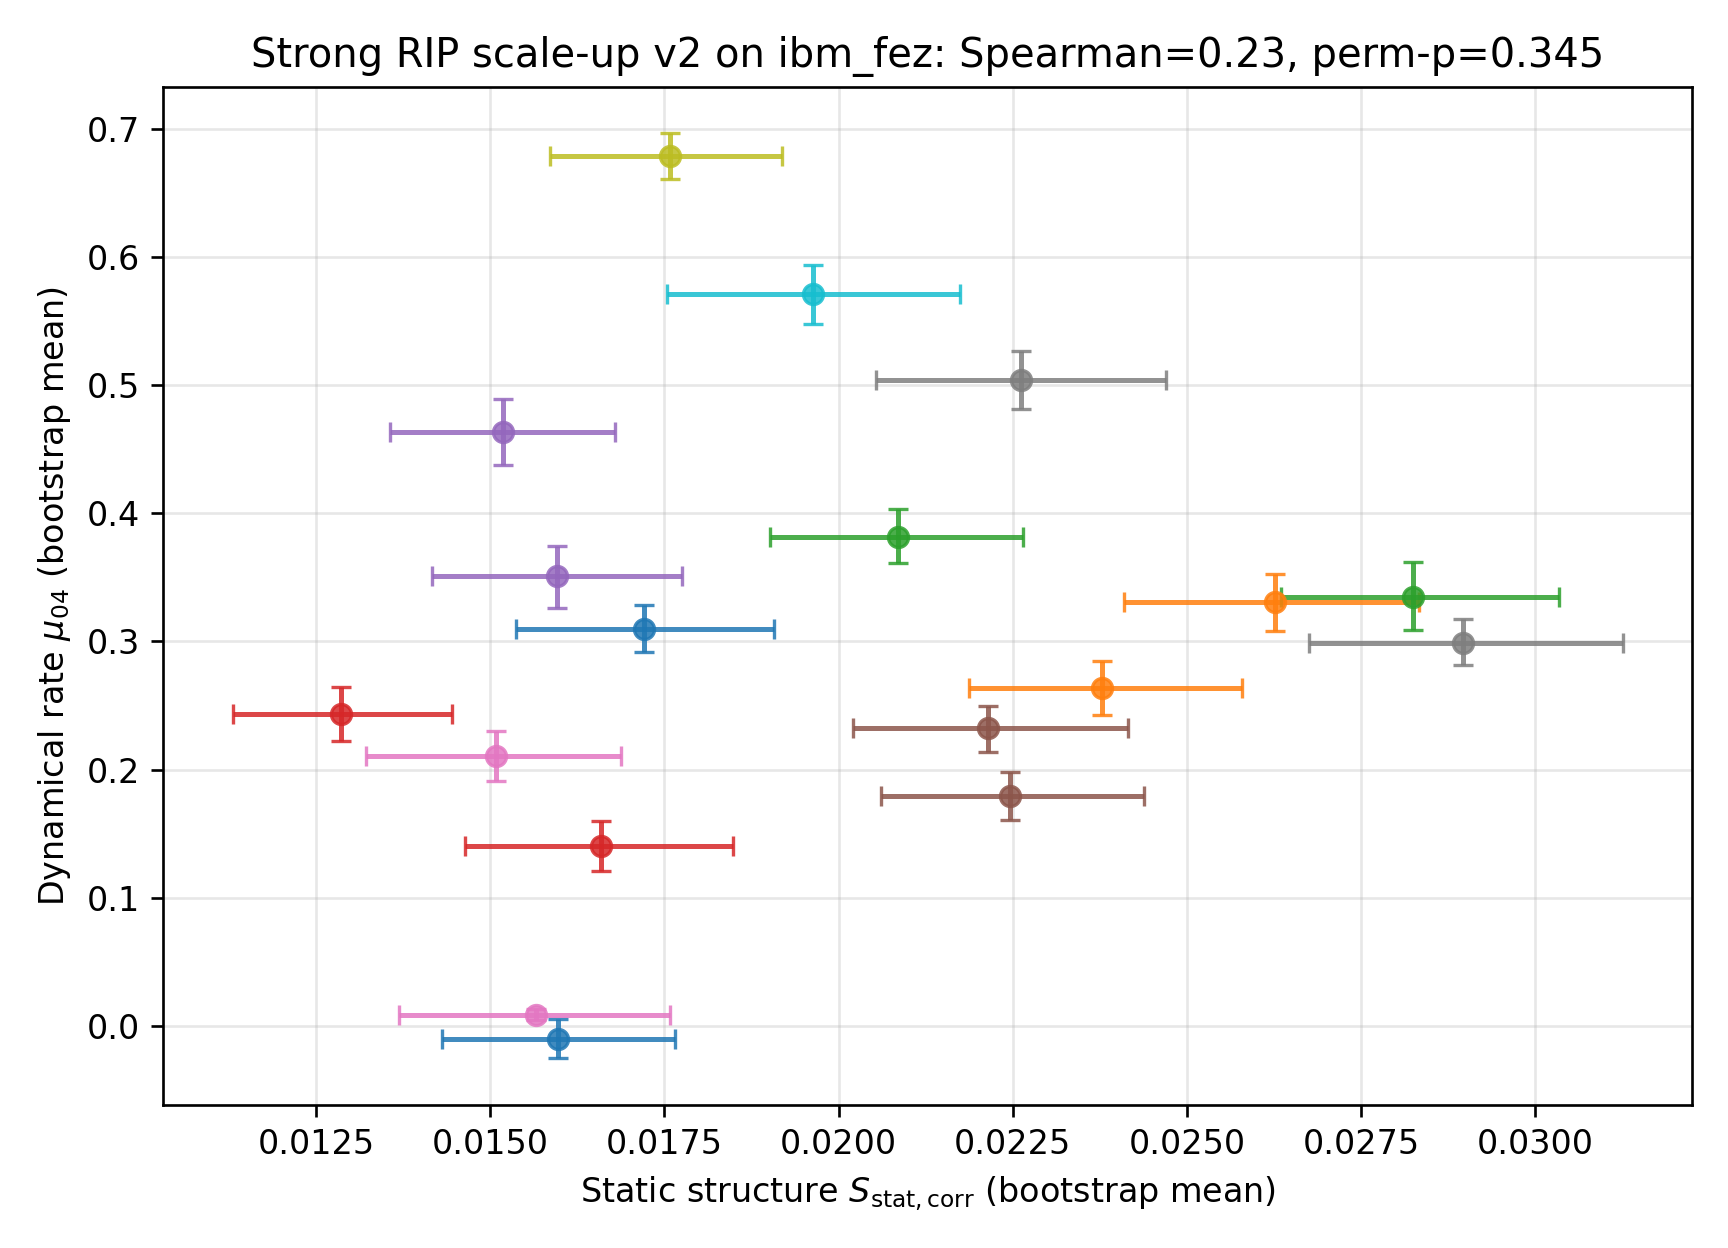
\includegraphics[width=0.75\textwidth]{rip_strong_scaleup_v2.png}
\caption{Scale-up v2 stress test ($n=18$ random chains): bootstrap means with
16--84\% intervals, $S_{\rm stat,corr}$ vs $\mu_{04}$.}
\label{fig:scaleup}
\end{figure}

\begin{table}[h]
\centering
\caption{Preregistered out-of-sample prediction test on \texttt{ibm\_fez}.}
\label{tab:prereg}
\begin{tabular}{lcl}
\hline
Group & $\overline{\mu_{04}}$ & Notes \\
\hline
LOW & 0.334723 & $k=5$ chains, smallest static metric \\
HIGH & 0.333317 & $k=5$ chains, largest static metric \\
\hline
\end{tabular}
\end{table}

\paragraph{Interpretation.} The curated three-chain set exhibits an ordering
agreement between the static Ramsey-X metric and the dynamical decay scales.
However, the scale-up and preregistered tests do not support a device-wide
monotone static--dynamic law under the present metrics and sampling, within
the power quantified above. Either (i) the dominant mechanisms determining
transport decay on generic chains are not captured by the Ramsey-X
nearest-neighbor covariance metric, or (ii) the relevant static predictor is
more mechanism-specific (e.g., two-qubit $ZZ$-type static probes on
transport edges), which is left for future work.

\section{Reproducibility artifacts}
\label{sec:repro}
All primary figures are generated from IBM Quantum Runtime job outputs
identified by the Job IDs in Section~2 and from the analysis scripts used in
the original runs. The processed JSON artifacts from v1
(\texttt{rip\_comparative\_fit\_v3\_fixB.json},
\texttt{rip\_strong\_scaleup\_v2.json},
\texttt{rip\_predictive\_dynamic.json}) were \emph{not} preserved outside
the provider account; therefore this release does not claim fully offline
reproduction of the on-device numbers. The Job IDs remain the primary data
reference, and job results remain retrievable through the IBM Quantum
account records (e.g.\ \texttt{service.job(<id>).result()} in
\texttt{qiskit-ibm-runtime}) while retained by the provider. The series
repository ships \texttt{verification/0105/reanalyze\_0105.py} with a
documented canonical JSON schema and a synthetic-data validation mode
(\texttt{--demo}), covering the fit-variant table, scale-up rank tests, the
preregistered statistic and its permutation $p$-values, the power analysis,
and the $\mu_{\rm all}$ proxy. A future data revision will populate
\texttt{results/0105/} -- ideally with raw per-circuit counts (chain id,
$L$, basis, repetition, timestamp) rather than processed summaries --
enabling full offline re-analysis. Unlike the other verification suites in
this series, this script \emph{re-analyzes archived measurements}; it
cannot regenerate them.

\section{Conclusion}
We reported (i) a replicated, high-resolution prefix-path Bell-transport
dataset on \texttt{ibm\_fez} and (ii) a comparative geometry test across
three disjoint physical chains, yielding $>10\sigma$ differences in an
effective decay scale $\mu$ under the stated fit protocol (ordering read as
the robust claim; see the fitting-choice caveat). We also investigated a candidate static--dynamic link: a
curated three-chain set exhibits an ordering agreement, but scale-up
analyses and a preregistered out-of-sample prediction test (adequately
powered against a strong device-wide law) do not show statistically significant association under the present
operationalization. We present the static--dynamic ordering agreement as
conditional and geometry-specific, and treat identification of a more
mechanism-aligned static predictor as an open experimental direction.

\section*{Note added in v2}
No experimental data changed; all Job IDs, figures and v1 numbers are
unchanged. v2 adds analysis-robustness and reproducibility layers:
(1) fitting-choice caveat (Section 5.3): the $B_{\rm fix}$ bias and the
ordering-stability of well-separated scales are demonstrated on synthetic
ground truth; the on-device variant table is deferred to a data revision;
(2) power bound for the negative preregistered test
(Section~\ref{sec:negative}): the design excludes a strong device-wide
static--dynamic law from published quantities alone, with the numerical MDE
deferred;
(3) all-lengths rate proxy $\mu_{\rm all}$ specified;
(4) small-sample caveats ($t$-factors for $n_{\rm rep}=3$ SEMs; no clipping
of the affine drift-corrected estimator);
(5) offline re-analysis script with documented schema and synthetic
validation (\texttt{reanalyze\_0105.py});
(6) context references on device error heterogeneity and crosstalk
\cite{Sarovar2020,Tripathi2022}.

\begin{thebibliography}{12}
\bibitem{NC} M.~A. Nielsen and I.~L. Chuang, \emph{Quantum Computation and
Quantum Information}, Cambridge University Press (2000).
\bibitem{BP} H.-P. Breuer and F. Petruccione, \emph{The Theory of Open
Quantum Systems}, Oxford University Press (2002).
\bibitem{Davies} E.~B. Davies, \emph{Markovian master equations}, Commun.
Math. Phys. \textbf{39} (1974) 91--110.
\bibitem{Petz} D. Petz, \emph{Sufficient subalgebras and the relative entropy
of states of a von Neumann algebra}, Commun. Math. Phys. \textbf{105} (1986)
123--131.
\bibitem{FR} O. Fawzi and R. Renner, \emph{Quantum conditional mutual
information and approximate Markov chains}, Commun. Math. Phys. \textbf{340}
(2015) 575--611.
\bibitem{RB} E. Magesan, J.~M. Gambetta, and J. Emerson, \emph{Scalable and
robust randomized benchmarking of quantum processes}, Phys. Rev. Lett.
\textbf{106} (2011) 180504.
\bibitem{Qiskit} Qiskit contributors, \emph{Qiskit: An Open-source Framework
for Quantum Computing}, \url{https://qiskit.org}.
\bibitem{Index} L. Eriksson, \emph{Coherence-maintenance program index},
\url{https://ai.vixra.org/author/lluis_eriksson}.
\bibitem{RIP0072} L. Eriksson, \emph{The Rate Inheritance Principle: From
Static Correlations to Dynamical Decoherence Rates}, ai.viXra:2512.0072
(2025).
\bibitem{RIP0070} L. Eriksson, \emph{Stress Testing the Rate Inheritance
Principle: Spectral Decoherence Rates and an Operational Resource Horizon},
ai.viXra:2512.0070 (2025).
\bibitem{Sarovar2020} M. Sarovar, T. Proctor, K. Rudinger, K. Young,
E. Nielsen, and R. Blume-Kohout, \emph{Detecting crosstalk errors in quantum
information processors}, Quantum \textbf{4} (2020) 321.
\bibitem{Tripathi2022} V. Tripathi, H. Chen, M. Khezri, K.-W. Yip,
E.~M. Levenson-Falk, and D.~A. Lidar, \emph{Suppression of crosstalk in
superconducting qubits using dynamical decoupling}, Phys. Rev. Applied
\textbf{18} (2022) 024068.
\end{thebibliography}

\end{document}
